\documentclass{ximeraXloud}
\usepackage{longdivision}
\usepackage{polynom}
\usepackage{float}% Use `H' as the figure optional argument to force it's vertical placement to conform to source.
%\usepackage{caption}% Allows us to describe the figures without having "figure 1:" in it. :: Apparently Caption isn't supported.
%    \captionsetup{labelformat=empty}% Actually does the figure configuration stated above.
\usetikzlibrary{arrows.meta,arrows}% Allow nicer arrow heads for tikz.
\usepackage{gensymb, pgfplots}
\usepackage{tabularx}
\usepackage{arydshln}



\graphicspath{
  {./}
  {./explorePolynomials/}
  {./exploreRadicals/}
  {./graphing/}
}

%% Default style for tikZ
\pgfplotsset{my style/.append style={axis x line=middle, axis y line=
middle, xlabel={$x$}, ylabel={$y$}, axis equal }}


%% Because log being natural log is too hard for people.
\let\logOld\log% Keep the old \log definition, just in case we need it.
\renewcommand{\log}{\ln}


%%% Changes in polynom to show the zero coefficient terms
\makeatletter
\def\pld@CF@loop#1+{%
    \ifx\relax#1\else
        \begingroup
          \pld@AccuSetX11%
          \def\pld@frac{{}{}}\let\pld@symbols\@empty\let\pld@vars\@empty
          \pld@false
          #1%
          \let\pld@temp\@empty
          \pld@AccuIfOne{}{\pld@AccuGet\pld@temp
                            \edef\pld@temp{\noexpand\pld@R\pld@temp}}%
           \pld@if \pld@Extend\pld@temp{\expandafter\pld@F\pld@frac}\fi
           \expandafter\pld@CF@loop@\pld@symbols\relax\@empty
           \expandafter\pld@CF@loop@\pld@vars\relax\@empty
           \ifx\@empty\pld@temp
               \def\pld@temp{\pld@R11}%
           \fi
          \global\let\@gtempa\pld@temp
        \endgroup
        \ifx\@empty\@gtempa\else
            \pld@ExtendPoly\pld@tempoly\@gtempa
        \fi
        \expandafter\pld@CF@loop
    \fi}
\def\pld@CMAddToTempoly{%
    \pld@AccuGet\pld@temp\edef\pld@temp{\noexpand\pld@R\pld@temp}%
    \pld@CondenseMonomials\pld@false\pld@symbols
    \ifx\pld@symbols\@empty \else
        \pld@ExtendPoly\pld@temp\pld@symbols
    \fi
    \ifx\pld@temp\@empty \else
        \pld@if
            \expandafter\pld@IfSum\expandafter{\pld@temp}%
                {\expandafter\def\expandafter\pld@temp\expandafter
                    {\expandafter\pld@F\expandafter{\pld@temp}{}}}%
                {}%
        \fi
        \pld@ExtendPoly\pld@tempoly\pld@temp
        \pld@Extend\pld@tempoly{\pld@monom}%
    \fi}
\makeatother




%%%%% Code for making prime factor trees for numbers, taken from user Qrrbrbirlbel at: https://tex.stackexchange.com/questions/131689/how-to-automatically-draw-tree-diagram-of-prime-factorization-with-latex

\usepackage{forest,mathtools,siunitx}
\makeatletter
\def\ifNum#1{\ifnum#1\relax
  \expandafter\pgfutil@firstoftwo\else
  \expandafter\pgfutil@secondoftwo\fi}
\forestset{
  num content/.style={
    delay={
      content/.expanded={\noexpand\num{\forestoption{content}}}}},
  pt@prime/.style={draw, circle},
  pt@start/.style={},
  pt@normal/.style={},
  start primeTree/.style={%
    /utils/exec=%
      % \pt@start holds the current minimum factor, we'll start with 2
      \def\pt@start{2}%
      % \pt@result will hold the to-be-typeset factorization, we'll start with
      % \pgfutil@gobble since we don't want a initial \times
      \let\pt@result\pgfutil@gobble
      % \pt@start@cnt holds the number of ^factors for the current factor
      \def\pt@start@cnt{0}%
      % \pt@lStart will later hold "l"ast factor used
      \let\pt@lStart\pgfutil@empty,
    alias=pt-start,
    pt@start/.try,
    delay={content/.expanded={$\noexpand\num{\forestove{content}}
                            \noexpand\mathrlap{{}= \noexpand\pt@result}$}},
    primeTree},
  primeTree/.code=%
    % take the content of the node and save it in the count
    \c@pgf@counta\forestove{content}\relax
    % if it's 2 we're already finished with the factorization
    \ifNum{\c@pgf@counta=2}{%
      % add the factor
      \pt@addfactor{2}%
      % finalize the factorization of the result
      \pt@addfactor{}%
      % and set the style to the prime style
      \forestset{pt@prime/.try}%
    }{%
      % this simply calculates content/2 and saves it in \pt@end
      % this is later used for an early break of the recursion since no factor
      % can be greater then content/2 (for integers of course)
      \edef\pt@content{\the\c@pgf@counta}%
      \divide\c@pgf@counta2\relax
      \advance\c@pgf@counta1\relax % to be on the safe side
      \edef\pt@end{\the\c@pgf@counta}%
      \pt@do}}

%%% our main "function"
\def\pt@do{%
  % let's test if the current factor is already greather then the max factor
  \ifNum{\pt@end<\pt@start}{%
    % great, we're finished, the same as above
    \expandafter\pt@addfactor\expandafter{\pt@content}%
    \pt@addfactor{}%
    \def\pt@next{\forestset{pt@prime/.try}}%
  }{%
    % this calculates int(content/factor)*factor
    % if factor is a factor of content (without remainder), the result will
    % equal content. The int(content/factor) is saved in \pgf@temp.
    \c@pgf@counta\pt@content\relax
    \divide\c@pgf@counta\pt@start\relax
    \edef\pgf@temp{\the\c@pgf@counta}%
    \multiply\c@pgf@counta\pt@start\relax
    \ifNum{\the\c@pgf@counta=\pt@content}{%
      % yeah, we found a factor, add it to the result and ...
      \expandafter\pt@addfactor\expandafter{\pt@start}%
      % ... add the factor as the first child with style pt@prime
      % and the result of int(content/factor) as another child.
      \edef\pt@next{\noexpand\forestset{%
        append={[\pt@start, pt@prime/.try]},
        append={[\pgf@temp, pt@normal/.try]},
        % forest is complex, this makes sure that for the second child, the
        % primeTree style is not executed too early (there must be a better way).
        delay={
          for descendants={
            delay={if n'=1{primeTree, num content}{}}}}}}%
    }{%
      % Alright this is not a factor, let's get the next factor
      \ifNum{\pt@start=2}{%
        % if the previous factor was 2, the next one will be 3
        \def\pt@start{3}%
      }{%
        % hmm, the previos factor was not 2,
        % let's add 2, maybe we'll hit the next prime number
        % and maybe a factor
        \c@pgf@counta\pt@start
        \advance\c@pgf@counta2\relax
        \edef\pt@start{\the\c@pgf@counta}%
      }%
      % let's do that again
      \let\pt@next\pt@do
    }%
  }%
  \pt@next
}

%%% this builds the \pt@result macro with the factors
\def\pt@addfactor#1{%
  \def\pgf@tempa{#1}%
  % is it the same factor as the previous one
  \ifx\pgf@tempa\pt@lStart
    % add 1 to the counter
    \c@pgf@counta\pt@start@cnt\relax
    \advance\c@pgf@counta1\relax
    \edef\pt@start@cnt{\the\c@pgf@counta}%
  \else
    % a new factor! Add the previous one to the product of factors
    \ifx\pt@lStart\pgfutil@empty\else
      % as long as there actually is one, the \ifnum makes sure we do not add ^1
      \edef\pgf@tempa{\noexpand\num{\pt@lStart}\ifnum\pt@start@cnt>1 
                                           ^{\noexpand\num{\pt@start@cnt}}\fi}%
      \expandafter\pt@addfactor@\expandafter{\pgf@tempa}%
    \fi
    % setup the macros for the next round
    \def\pt@lStart{#1}% <- current (new) factor
    \def\pt@start@cnt{1}% <- first time
  \fi
}
%%% This simply appends "\times #1" to \pt@result, with etoolbox this would be
%%% \appto\pt@result{\times#1}
\def\pt@addfactor@#1{%
  \expandafter\def\expandafter\pt@result\expandafter{\pt@result \times #1}}

%%% Our main macro:
%%% #1 = possible optional argument for forest (can be tikz too)
%%% #2 = the number to factorize
\newcommand*{\PrimeTree}[2][]{%
  \begin{forest}%
    % as the result is set via \mathrlap it doesn't update the bounding box
    % let's fix this:
    tikz={execute at end scope={\pgfmathparse{width("${}=\pt@result$")}%
                         \path ([xshift=\pgfmathresult pt]pt-start.east);}},
    % other optional arguments
    #1
    % And go!
    [#2, start primeTree]
  \end{forest}}
\makeatother


\providecommand\tabitem{\makebox[1em][r]{\textbullet~}}
\providecommand{\letterPlus}{\makebox[0pt][l]{$+$}}
\providecommand{\letterMinus}{\makebox[0pt][l]{$-$}}



\title{Polynomial Synthetic Division}
\begin{document}
\begin{abstract}
    Factor out a polynomial using synthetic division
\end{abstract}%
\maketitle

Here is a shortcut method that computes the polynomial long division in \textit{specific circumstances}. Often this method, synthetic division, ends up getting used when it shouldn't because it is (in some ways) easier and faster, so it becomes the primary tool for students and they forget polynomial long division. Even more of an issue however is that the \textit{circumstances} when one \textit{must} use polynomial long division rather than synthetic division is also often forgotten.

Synthetic division is appropriate when you want to divide out a degree one real root. Specifically if you have a root \textit{purely of the form }$(x-c)$ for some real number $c$. Notice that this means we must have $1$ as a coefficient in front of the $x$ and we can't use synthetic division to remove a root which is an irreducible quadratic.%
\footnote{%
    Technically $c$ doesn't \textit{have} to be a real number, it could be a complex number. \textit{However} in practice the computation becomes a bit of a nightmare and almost always ends up incorrect. For this reason I would \textbf{strongly} suggest not using synthetic division when you have a complex root. In fact, one should not do polynomial \textit{or} synthetic division with complex valued roots as there is a much better way to tackle that situation which we will discuss later.%
    }

Synthetic division is not dissimilar from polynomial long division, but we omit the powers of $x$. In essence, instead of copying down the polynomial (remembering to use a coefficient of zero for any missing powers of $x$), we write down the coefficients only, in a grid-like pattern, and then instead of writing along the top a polynomial that includes powers of $x$ we will write the coefficients only.

The advantage to doing this, is that the algorithm for computing the number you need becomes a bit simpler. It turns out that the coefficients you need to use can be determined through a pattern of addition and multiplication rather than division and subtraction... this is because division and multiplication are really the same thing (multiplying by a fraction and dividing by the inverse of that fraction are the same for instance), as are addition and subtracting (adding a negative is the same as subtracting the positive). But often this is easier for you to compute quickly because of how much human brains like to add and multiply instead of divide and subtract. Consider the following example;

\begin{image}
    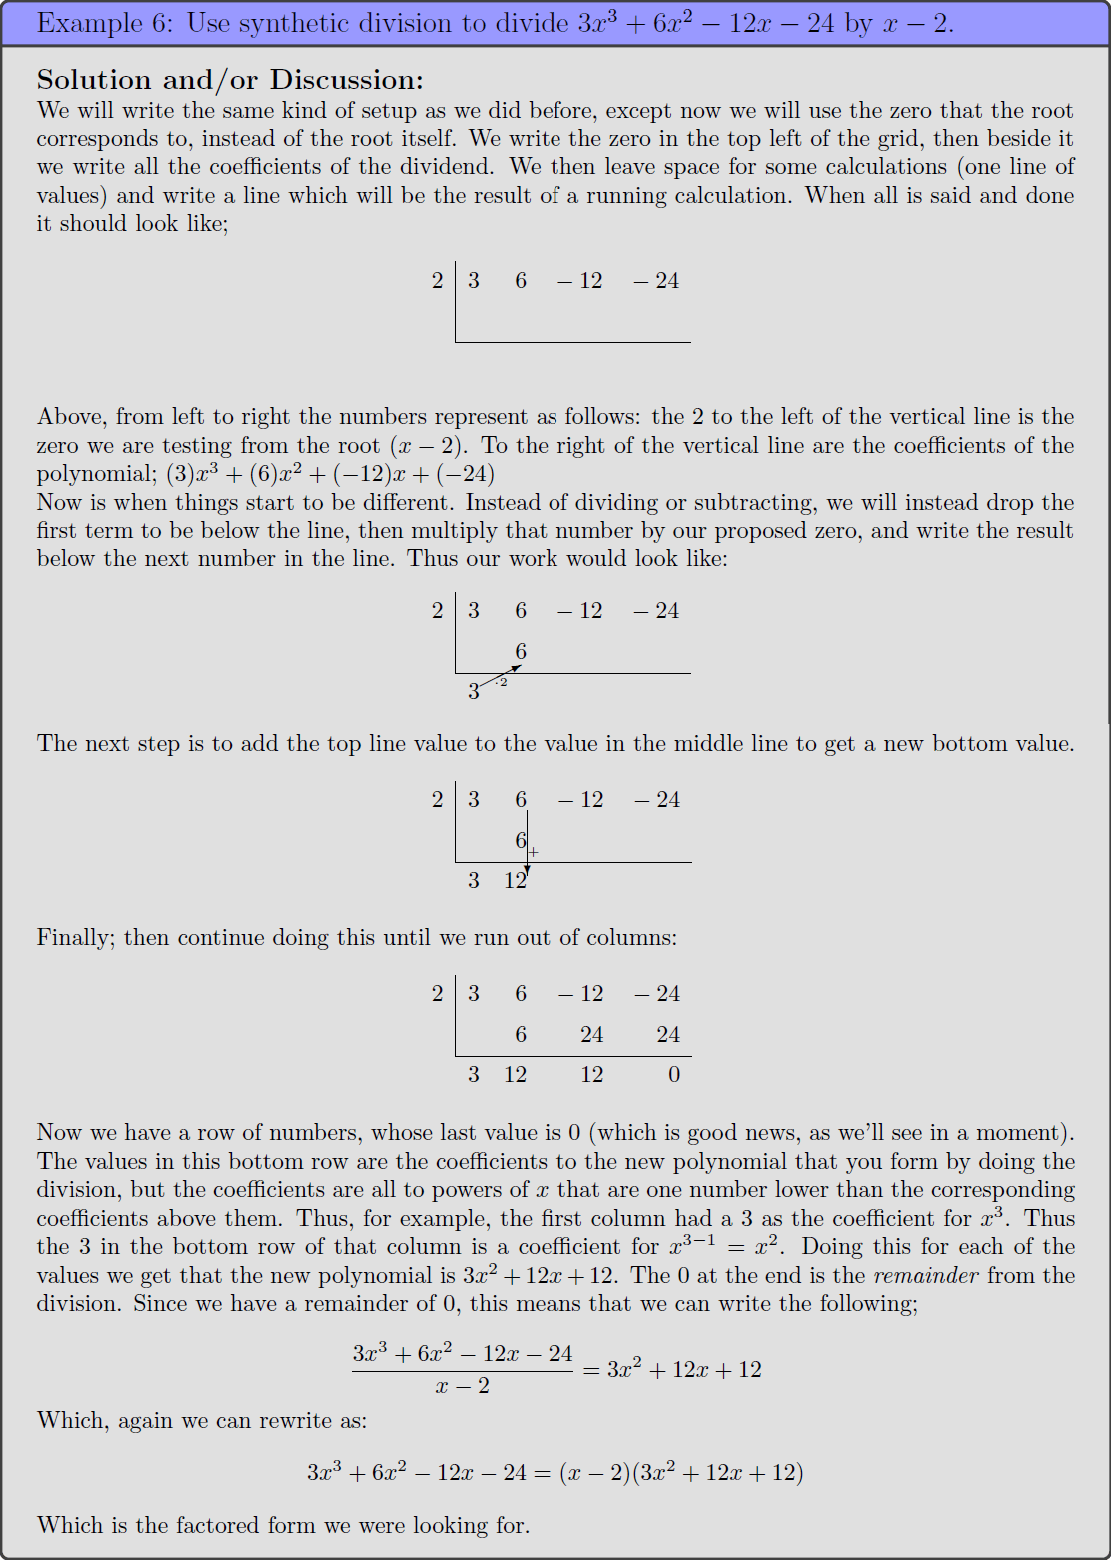
\includegraphics[width=\textwidth]{exPolySyntheticDivision.png}
\end{image}%


You can also watch a walkthrough of using polynomial synthetic division and its parallels to polynomial long division!

\youtube{aV_gOAKWCKM}

%\begin{example}%
%    Use synthetic division to divide $3x^3 + 6x^2 - 12x - 24$ by $x - 2$.\\
%    
%    We will write the same kind of setup as we did before, except now we will use the zero that the root corresponds to, instead of the root itself. We write the zero in the top left of the grid, then beside it we write all the coefficients of the dividend. We then leave space for some calculations (one line of values) and write a line which will be the result of a running calculation. When all is said and done it should look like; 
%    
%    \begin{center}
%        \polyhornerscheme[showbase=top,stage=1,x=2]{3x^3 + 6x^2 - 12x - 24}
%    \end{center}
%    
%    Above, from left to right the numbers represent as follows: the $2$ to the left of the vertical line is the zero we are testing from the root $(x-2)$. To the right of the vertical line are the coefficients of the polynomial; $(3)x^3 + (6)x^2 + (-12)x + (-24)$
%    
%    Now is when things start to be different. Instead of dividing or subtracting, we will instead drop the first term to be below the line, then multiply that number by our proposed zero, and write the result below the next number in the line. Thus our work would look like:
%    
%    \begin{center}
%        \polyhornerscheme[showbase=top,stage=3,tutor=true,x=2]{3x^3 + 6x^2 - 12x - 24}
%    \end{center}
%    
%    The next step is to add the top line value to the value in the middle line to get a new bottom value.
%    
%    \begin{center}
%        \polyhornerscheme[showbase=top,stage=4,tutor=true,x=2]{3x^3 + 6x^2 - 12x - 24}
%    \end{center}
%    
%    Finally; then continue doing this until we run out of columns:
%    
%    \begin{center}
%        \polyhornerscheme[showbase=top,x=2]{3x^3 + 6x^2 - 12x - 24}
%    \end{center}
%    
%    Now we have a row of numbers, whose last value is 0 (which is good news, as we'll see in a moment). The values in this bottom row are the coefficients to the new polynomial that you form by doing the division, but the coefficients are all to powers of $x$ that are one number lower than the corresponding coefficients above them. Thus, for example, the first column had a $3$ as the coefficient for $x^3$. Thus the $3$ in the bottom row of that column is a coefficient for $x^{3-1} = x^2$. Doing this for each of the values we get that the new polynomial is $3x^2 + 12x + 12$. The $0$ at the end is the \textit{remainder} from the division. Since we have a remainder of $0$, this means that we can write the following;
%
%    \[
%        \dfrac{3x^3 + 6x^2 - 12x - 24}{x-2} = 3x^2 + 12x + 12
%    \]
%    
%    Which, again we can rewrite as:
%    \[
%        3x^3 + 6x^2 - 12x - 24 = (x-2)(3x^2 + 12x + 12)
%    \]
%    
%    Which is the factored form we were looking for.
%    \end{example}% End Example.

\end{document}